\documentclass{izpit}
% Paket lahko naložite z neobveznimi možnostmi:
% - arhiv:
%     Izpis, namenjen za objavo izpita v arhivu. Naloge se pišejo ena pod
%     drugo, brez vmesnega prostora za reševanje, v glavi pa ni vpisnih polj.
% - izpolnjen:
%     Izpis, namenjen za generirane domače naloge. V glavi ni vpisnih polj,
%     saj se predpostavlja, da so že izpolnjena (vsak študent ima svojo
%     verzijo)
% - brezpaketov:
%     Prepreči nalaganje paketov amsmath, amssym, babel in inputenc. To
%     možnost uporabite, če je kakšen od teh paketov v konfliktu z vašimi.
%     Paketi ifthen, keyval, geometry in tikz se vedno naložijo, saj so
%     za uporabo paketa izpit obvezni.
% - sumniki:
%     Če vaš urejevalnik pod Windowsi ne pozna kodne tabele UTF-8
%     (ostali operacijski sistemi že leta podpirajo UTF-8),
%     uporabite možnost sumniki, da boste lahko pisali č namesto "c, ali \v c.
% - 10pt, 11pt, fleqn, ...
%     Uporabite lahko tudi vse ostale možnosti ki obstajajo v paketu article.
%     V osnovi je velikost črk 11pt.

\begin{document}

%==========================================================================
%               Sem vpisi stevila tock in bo latex naracunal procente
%==========================================================================
\FRACTIONSIMPLIFY{60}{1}{\skupnotock}{\nepomembno}% zal se v paketu ne da enostavneje shraniti
\MAX{0.1}{0}{\tempepsilon}%shranimo epsilon... ne gre trik z ulomkom zato max
%\ADD{\skupnotock}{\tockecetrte}{\skupnotock}%ce dodajamo dodatno nalogo
\DIVIDE{\skupnotock}{10}{\sol}
\MULTIPLY{\sol}{9}{\odlicno}
\MULTIPLY{\sol}{7.6}{\pravdobro}
\MULTIPLY{\sol}{6.3}{\dobro}
\MULTIPLY{\sol}{5}{\zadostno}
\ADD{\dobro}{\tempepsilon}{\dobroplus}%dodajanje epsilonov v spodnje meje
\ADD{\pravdobro}{\tempepsilon}{\pravdobroplus}
\ADD{\odlicno}{\tempepsilon}{\odlicnoplus}
\ROUND[1]{\dobroplus}{\dobroplus}%zaokrozevanje
\ROUND[1]{\pravdobroplus}{\pravdobroplus}
\ROUND[1]{\odlicnoplus}{\odlicnoplus}
\ROUND[1]{\zadostno}{\zadostno}
\ROUND[1]{\dobro}{\dobro}
\ROUND[1]{\pravdobro}{\pravdobro}
\ROUND[1]{\odlicno}{\odlicno}
%==========================================================================
%               Sem vpisi podatke o izpitu (ucilnica = RAZRED ali JEDILNICA)
%==========================================================================
\izpit[ucilnica = RAZRED, naloge = 4, brez vpisne]%ucilnica RAZRED,JEDILNICA, lahko se sedezni red
{Matematika - Polinomi}{30. 9. 2239}{Čas pisanja je 45 minut.\\ Možno je doseči $\skupnotock$ točk.\\ Veliko uspeha!}

 %%%%%%%%%%%%%%%%%%%%
 \PlaceText{100mm}{40mm}{\begin{tabular}{ll}
    \multicolumn{2}{c}{\textbf{Kriterij ocenjevanja}} \\[0.5ex]
    Ocena & Tocke \\ \hline
    zadostno & $\zadostno - \dobro$ \\
    dobro & $\dobroplus - \pravdobro$ \\
    prav dobro & $\pravdobroplus - \odlicno$ \\
    odlicno & $\odlicnoplus$--
  \end{tabular}}
%==========================================================================
%               Sem vpisi naloge
%   za dodatek koordinatnega sistema daj pod navodila naloge \[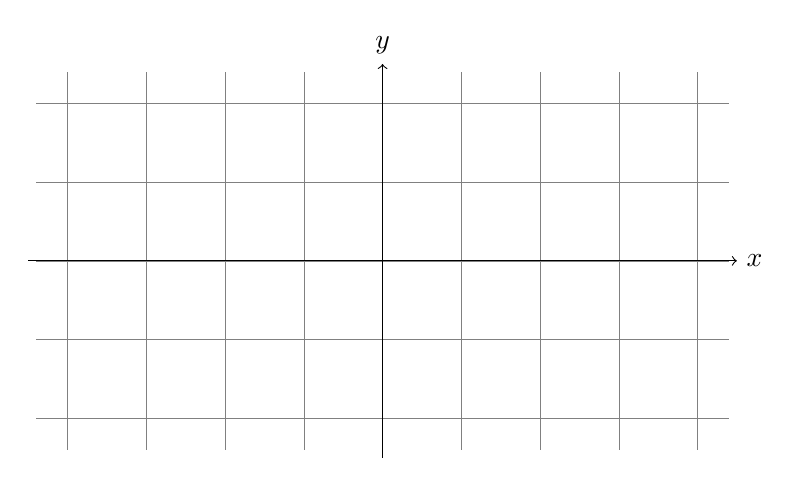
\begin{tikzpicture}
        \draw[help lines,step=1cm] (-4.4,-2.4) grid (4.4,2.4);
        \draw[->] (-4.5,0) -- (4.5,0) node[right] {$x$};
        \draw[->] (0,-2.5) -- (0,2.5) node[above] {$y$};
\end{tikzpicture}\]
%   oz. za kompleksno ravnino \[\begin{tikzpicture}
        \draw[help lines,step=1cm] (-4.4,-2.4) grid (4.4,2.4);
        \draw[->] (-4.5,0) -- (4.5,0) node[right] {$Re$};
        \draw[->] (0,-2.5) -- (0,2.5) node[above] {$Im$};
\end{tikzpicture}\]
%==========================================================================
  
\naloga[\tocke{25}]

%\[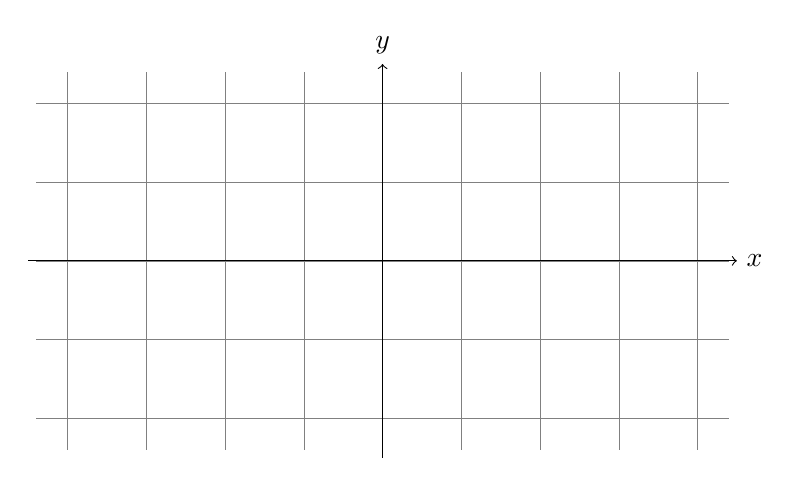
\begin{tikzpicture}
        \draw[help lines,step=1cm] (-4.4,-2.4) grid (4.4,2.4);
        \draw[->] (-4.5,0) -- (4.5,0) node[right] {$x$};
        \draw[->] (0,-2.5) -- (0,2.5) node[above] {$y$};
\end{tikzpicture}\]\\
\dodatek{\[\begin{tikzpicture}
        \draw[help lines,step=1cm] (-4.4,-2.4) grid (4.4,2.4);
        \draw[->] (-4.5,0) -- (4.5,0) node[right] {$Re$};
        \draw[->] (0,-2.5) -- (0,2.5) node[above] {$Im$};
\end{tikzpicture}\]}


\naloga[\tocke{20}]

  \podnaloga[15]
    Poiščite izjavo $X = X(p, q, r)$, ki ima naslednjo pravilnostno tabelo.
    Izjavo poenostavite do oblike, ki vsebuje kvečjemu dva logična veznika.
    \[
      \begin{tabular}{c|cccccccc}
        $p$ & 1 & 1 & 1 & 1 & 0 & 0 & 0 & 0 \\
        $q$ & 1 & 1 & 0 & 0 & 1 & 1 & 0 & 0 \\
        $r$ & 1 & 0 & 1 & 0 & 1 & 0 & 1 & 0 \\\hline
        $X$ & 1 & 0 & 1 & 0 & 1 & 0 & 1 & 1 \\
      \end{tabular}
    \]
  
  % Ukaz \prostor na polo doda prostor za rešitev. Ukaz sprejme neobvezen
  % argument, ki pove, kolikšen delež prostora naj bo namenjen nalogi.
  % Če paket naložite z možnostjo 'arhiv', ukaz \prostor ne naredi ničesar.
  \prostor[2] % Za to nalogo bo dvakrat toliko prostora kot za naslednjo.

  \podnaloga[5]
    Naj bo $G$ grupa in $H$ njena podgrupa edinka. Dokažite, da grupa $G$ ni
    enostavna natanko tedaj, ko ima $H$ polbrata.

  \prostor

\naloga[\tocke{16}]
  Skicirajte graf funkcije $f \colon \mathbb{R} \to \mathbb{R}$, podane s
  predpisom
  \[
    f(x) = \frac{1 + x - x^2}{3 x^2 - 5} \;.
  \]

  % Ukaz \dodatek uporabite, kadar na izpit želite dati sliko, tabelo, ali kaj
  % podobnega, kar bo študentom v pomoč pri pisanju odgovorov.
  % Če paket naložite z možnostjo 'arhiv', ukaz \dodatek ne naredi ničesar.
  \dodatek{\[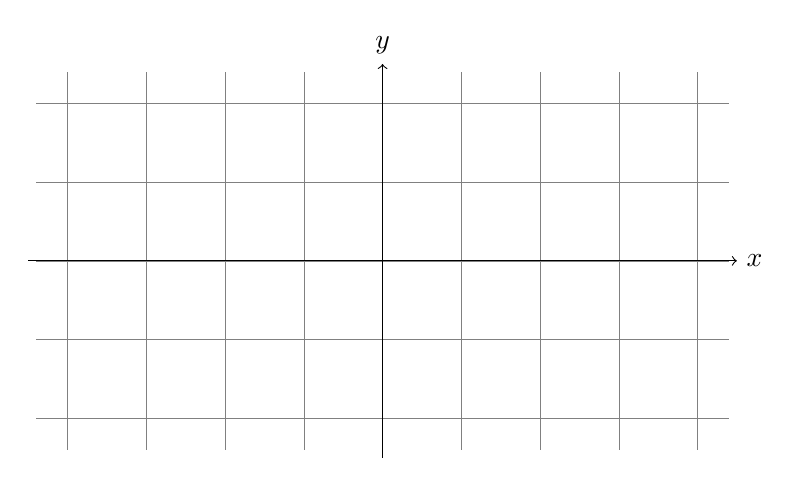
\begin{tikzpicture}
        \draw[help lines,step=1cm] (-4.4,-2.4) grid (4.4,2.4);
        \draw[->] (-4.5,0) -- (4.5,0) node[right] {$x$};
        \draw[->] (0,-2.5) -- (0,2.5) node[above] {$y$};
\end{tikzpicture}\]}

% Vsaka naslednja naloga gre v osnovi na novo stran. Če želite nalogo dodati
% na isto stran, uporabite ukaz \naloga*, ki se obnaša enako kot \naloga, le
% da ne naredi nove strani.
\naloga*[dodatnih 5 točk]%se ne steje v procente za ocene

  Za katera cela števila $c$ ima diofantska enačba
  \[
    72 x + 19 y = c
  \]
  rešitve v celih številih? Kakšna je v tem primeru splošna oblika rešitve?

\end{document}